\chapter{Testing} % Main chapter title
Una vez analizados todos los casos de estudios con sus respectivas particularidades, se logró un algoritmo conforme con las especificaciones necesarias antes definidas. Una vez alcanzado el mismo se decidió poner a prueba su desempeño ante nuevos escenarios.\\
Para cada uno de estos nuevos escenarios se llevo a cabo el mismo análisis realizado para los casos de estudio anteriores, sin embargo para no ser reiterativos en este aspecto no se especifican la totalidad de los pasos hasta resolver el deadlock, dado que ya han sido mencionados en el desarrollo de la investigación.

\section{Nuevos escenarios}

%-------------------------------------------------------------------------------------

\subsection{Caso Auto y Hiuxia}
Estas redes modelan la ejecución concurrente de un AMS.
En las mismas existen plazas que simulan la disponibilidad de recursos (3) y un control incorrecto de estos en la ejecución de los procesos de trabajo, puede conducir a situaciones de deadlock.\\
Un problema AMS consiste en un conjunto de recursos finitos como máquinas, búferes y robots. Diferentes tipos de piezas ingresan al sistema en momentos discretos y se procesan simultáneamente. Todas las partes procesadas en el sistema compiten por estos recursos finitos; por lo tanto, pueden producirse problemas como bloqueos, conflictos e interbloqueos. 

\subsubsection{Características generales red Auto}
\begin{itemize}
    \item Los recursos de la red están representados por las plazas \{$P_{19},P_{20},P_{21}$\}.
\end{itemize}

\subsubsection{Análisis estructural Auto}
\hfill
\begin{figure} [H]
	\centering
	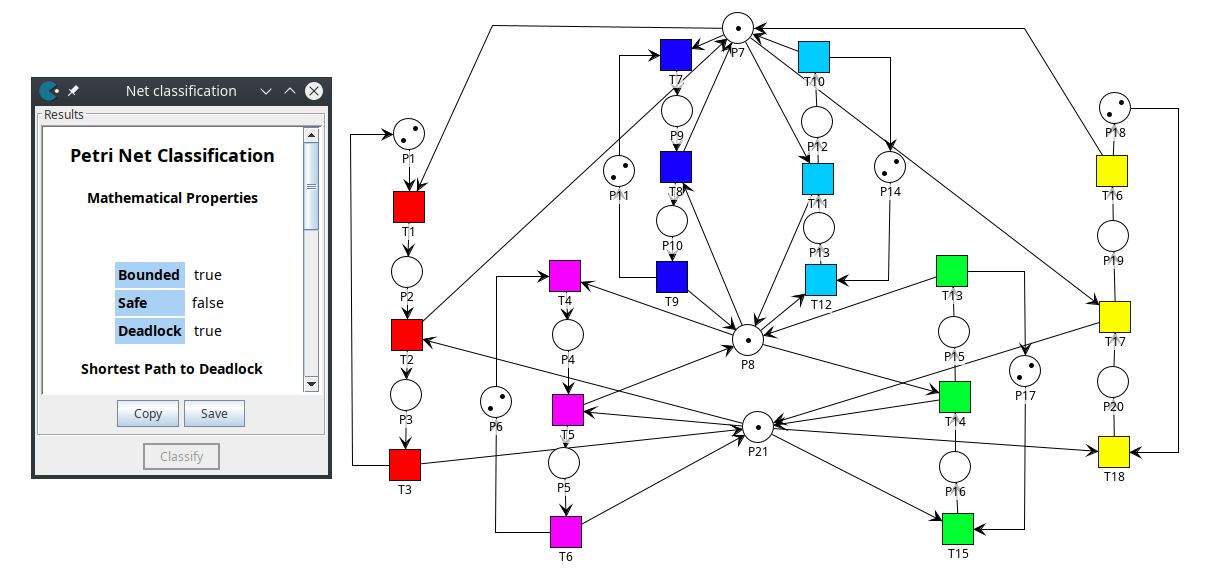
\includegraphics[width=\textwidth]{Figures/testing/auto-t-inv.png}
	\caption[RdP Auto y sus T-invariantes.]{RdP Auto \footnotemark \ y sus T-invariantes.}
	\label{fig:amsinvariantes}
 \end{figure} \footnotetext{Figura adaptada del paper publicado por \textit{Huixia Liu} et al. \cite{paperauto}}

En la figura \ref{fig:amsinvariantes}, se presentan los T-invariantes en diferentes colores. 

\paragraph{Control de la red}
\hfill \break
Al agregar los supervisores en la red ésta aún presentaba deadlock, lo que se hizo fue ejecutar la parte 3 del algoritmo para resolver tanto el problema de conflicto y de t\_idle, logrando de esta manera el control de la red.

\bigskip 
\begin{table}[H]
    \small
    \centering
    \begin{tabular}{|c|c|P{2cm}|P{2.3cm}|P{4.25cm}|}
    \hline
    \textbf{Supervisor} & \textbf{Marcado} & \textbf{Transiciones input} & \textbf{Transiciones output} & \textbf{Bad Siphon Controlado}  \\  \hline
    $P_{22}$ & 1 & \{$T_{2},T_{8},T_{11}, \break T_{13}$\} & \{$T_{1},T_{7},T_{12},T_{15}$\} & \{$P_2, P_5, P_9, P_{10}, P_{13}, P_{17}, \break P_{19}, P_{20}$\} \\ 
    \hline
    $P_{23}$ & 1 & \{$T_{2},T_{13},T_{17}$\} & \{$T_{1},T_{15},T_{18}$\} & \{$P_3, P_6, P_8, P_{10}, P_{14}, P_{17}, \break P_{19}, P_{21}$\} \\ 
    \hline
    $P_{24}$ & 1 & \{$T_{2},T_{5},T_{14}$\} & \{$T_{1},T_{4},T_{15}$\} & \{$P_3, P_6, P_9, P_{11}, P_{13}, P_{16}, \break P_{20}, P_{21}$\} \\ 
    \hline
    $P_{25}$ & 2 & \{$T_{2},T_{5},T_{8}, \break T_{11},T_{14},T_{17}$\} & \{$T_{1},T_{4},T_{7},T_{12}, \break T_{15},T_{18}$\} & \{$P_3, P_6, P_9, P_{10}, P_{13}, P_{17}, \break P_{19}, P_{20}, P_{21}$\} \\
    \hline
    \end{tabular}
    \caption{Supervisores: RdP Auto}
    \label{tab:AMS12-v4}
\end{table}
\hfill

\begin{figure}[H]
	\centering
	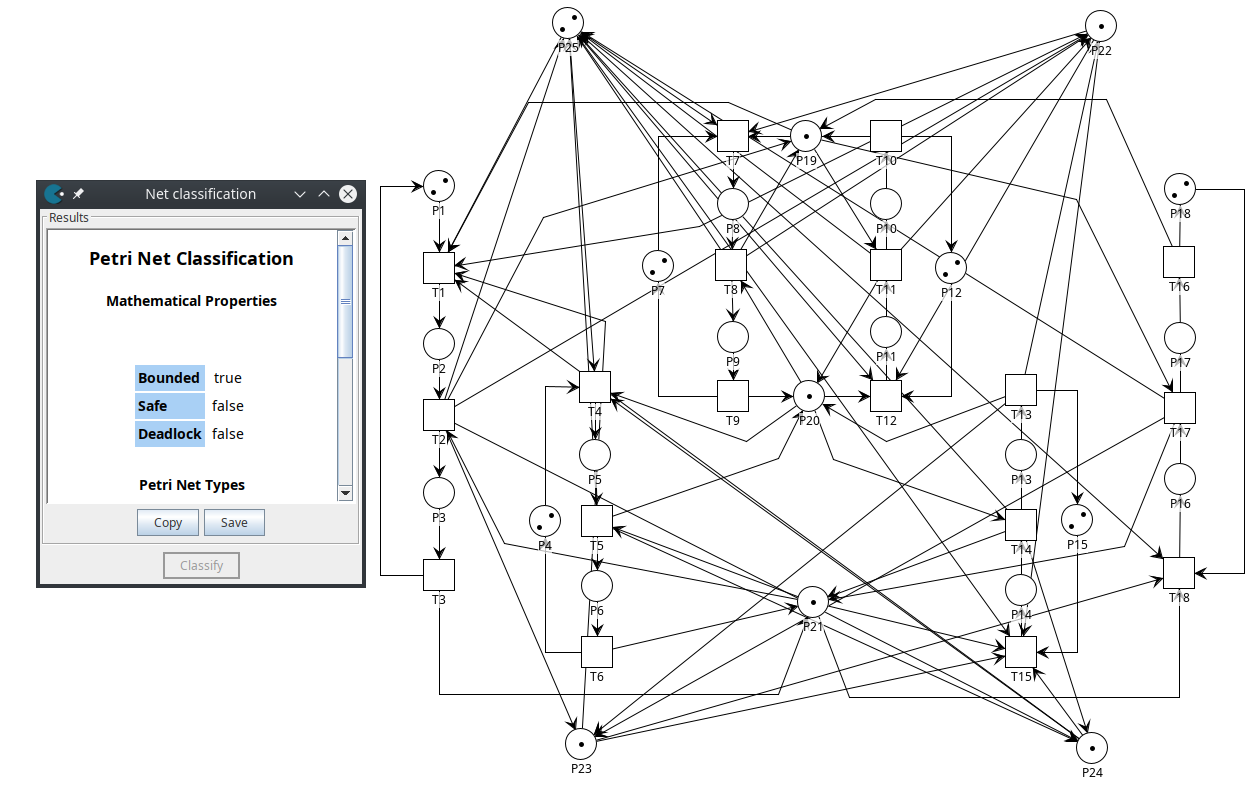
\includegraphics[scale=0.45]{Figures/testing/auto-controlada.png}
	\caption[RdP Auto controlada]{RdP Auto controlada.}
	\label{fig:amscontrolada}
 \end{figure} 

%-------------------------------------------------------------------------------

\subsubsection{Características generales red Hiuxia}
\begin{itemize}
    \item Los recursos de la red están representados por las plazas \{$P_{9},P_{10},P_{11}$\}.
\end{itemize}

\subsubsection{Análisis estructural red Hiuxia}
\hfill
\begin{figure}[H]
	\centering
	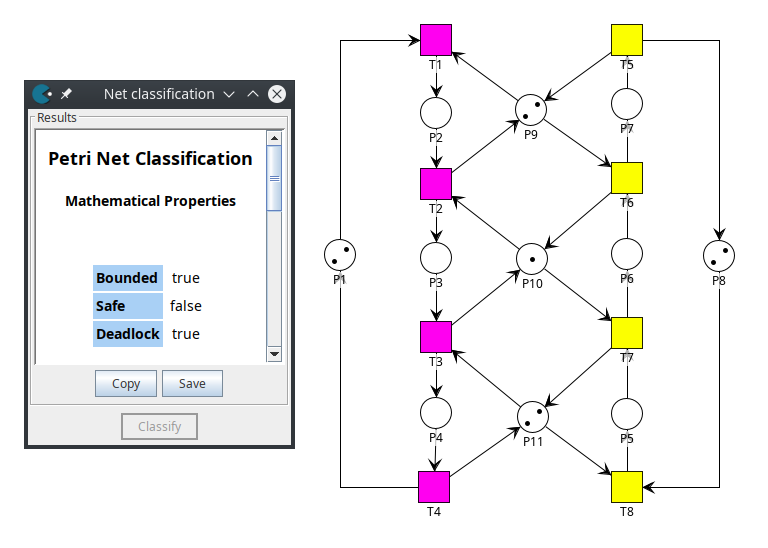
\includegraphics[scale=0.6]{Figures/testing/hiuxia-t-inv.png}
	\caption[RdP Hiuxia y sus T-invariantes.]{RdP Hiuxia \footnotemark \ y sus T-invariantes.}
	\label{fig:hiuxiainvariantes}
 \end{figure} \footnotetext{Figura adaptada del paper publicado por \textit{Huixia Liu} et al. \cite{paperauto}}

En la figura \ref{fig:hiuxiainvariantes}, se presentan los T-invariantes en diferentes colores. \\

\paragraph{Control de la red}
\hfill \break
Para alcanzar la vivacidad de esta red bastó con agregar los supervisores y no fue necesario ejecutar la parte 3 del algoritmo dado que al agregar los mismos se alcanzó el control de la red, eliminando las situaciones de deadlock.

\begin{table}[H]
    \small
    \centering
    \begin{tabular}{|c|c|P{2cm}|P{2.3cm}|c|}
    \hline
    \textbf{Supervisor} & \textbf{Marcado} & \textbf{Transiciones input} & \textbf{Transiciones output} & \textbf{Bad Siphon Controlado}  \\  \hline
    $P_{12}$ & 2 & \{$T_{2},T_{6}$\} & \{$T_{1},T_{8}$\} & \{$P_3, P_7, P_9, P_{10}$\} \\ 
    \hline
    $P_{13}$ & 2 & \{$T_{3}, T_{7}$\} & \{$T_1,T_8$\} & \{$P_4, P_6, P_{10}, P_{11}$\} \\ 
    \hline
    \end{tabular}
    \caption{Supervisores: RdP Hiuxia}
    \label{tab:Hiuxia12-v4}
\end{table}
\hfill

\begin{figure}[H]
	\centering
	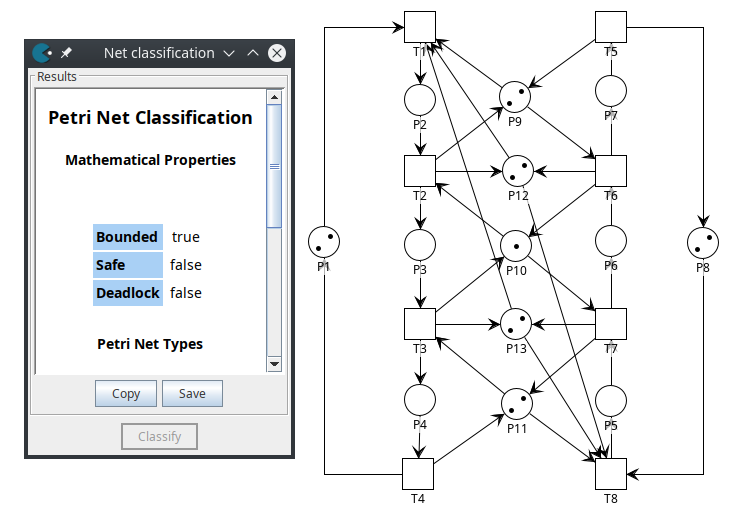
\includegraphics[width=\textwidth]{Figures/testing/hiuxia-controlada.png}
	\caption[RdP Hiuxia controlada]{RdP Hiuxia controlada.}
	\label{fig:hiuxiacontrolada}
 \end{figure} 
 
%-------------------------------------------------------------------------------------

\subsection{Casos YiFan (1,2,3) }
Estas tres redes\footnote{En estas RdP fueron modificados los pesos de los arcos reduciéndolos a uno para adaptarlas al tipo de red que admite el algoritmo.} presentes en el paper de YiFan et al. \cite{paperyifanhou} también son del tipo AMS. Este sistema consiste en un conjunto de estaciones interconectadas para el procesamiento de materiales que es capaz de procesar automáticamente una amplia variedad de tipos de piezas de manera simultánea y controlada por computadoras.\\
Un AMS tiene características de alto grado de automatización, de integración y de flexibilidad. 
En las redes existen ciertas plazas que simulan la disponibilidad de recursos y un control incorrecto de estos en la ejecución de los procesos de trabajo, puede conducir a situaciones de deadlock.

\subsubsection{Características generales YiFan1}
\begin{itemize}
    \item Los recursos de la red están representados por las plazas \{$P_{12},P_{13},P_{14}, P_{15}$\}.
\end{itemize}

\subsubsection{Análisis estructural YiFan1}
\hfill
\begin{figure}[H]
	\centering
	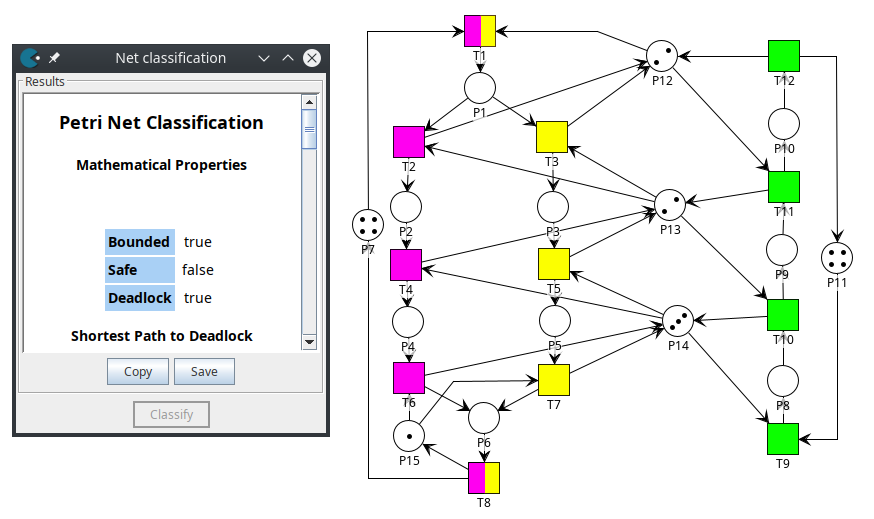
\includegraphics[width=\textwidth]{Figures/testing/yifan1_tinvariantes.png}
	\caption[RdP YiFan1 y sus T-invariantes.]{RdP YiFan1 \footnotemark \ y sus T-invariantes.}
	\label{fig:yifan1_invariantes}
 \end{figure} \footnotetext{Figura adaptada del paper publicado por \textit{YiFan Hou} et al. \cite{paperyifanhou}}

En la figura \ref{fig:yifan1_invariantes}, se presentan los diferentes T-invariantes en diferentes colores. \\

\paragraph{Control de la red}
\hfill \break
Para alcanzar la vivacidad de esta red bastó con agregar los supervisores y no fue necesario ejecutar la parte 3 del algoritmo dado que al agregar los mismos se alcanzó el control de la red, eliminando las situaciones de deadlock.

\bigskip
\begin{table}[H]
    \small
    \centering
    \begin{tabular}{|c|c|P{2cm}|P{2.3cm}|c|}
    \hline
    \textbf{Supervisor} & \textbf{Marcado} & \textbf{Transiciones input} & \textbf{Transiciones output} & \textbf{Bad Siphon Controlado}  \\  \hline
    $P_{16}$ & 3 & \{$T_{2},T_{3},T_{11}$\} & \{$T_{1},T_{9}$\} & \{$P_2, P_3, P_{10}, P_{12}, P_{13}$\} \\ 
    \hline
    $P_{17}$ & 4 & \{$T_{4}, T_{5}, T_{10}$\} & \{$T_1,T_9$\} & \{$P_4, P_5, P_{9}, P_{13}, P_{14}$\} \\ 
    \hline
    \end{tabular}
    \caption{Supervisores: RdP YiFan1}
    \label{tab:Yifan1}
\end{table}
\hfill

\begin{figure}[H]
	\centering
	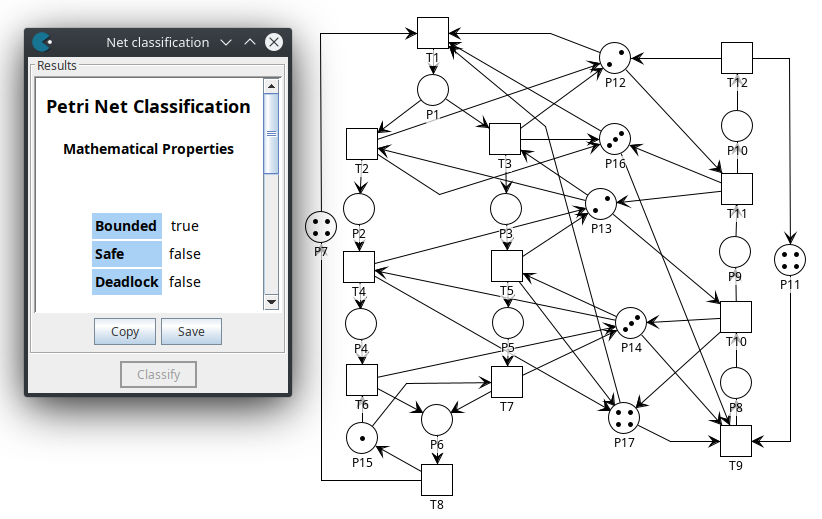
\includegraphics[width=\textwidth]{Figures/testing/yifan1_controlada.png}
	\caption[RdP YiFan1 controlada]{RdP YiFan1 controlada.}
	\label{fig:yifan1controlada}
 \end{figure}
 
 %-------------------------------------------------------------------------------------
\subsubsection{Características generales YiFan2}
\begin{itemize}
    \item Los recursos de la red están representados por las plazas \{$P_{11},P_{12},P_{13}$\}.
\end{itemize}

\subsubsection{Análisis estructural YiFan2}
\hfill
\begin{figure}[H]
	\centering
	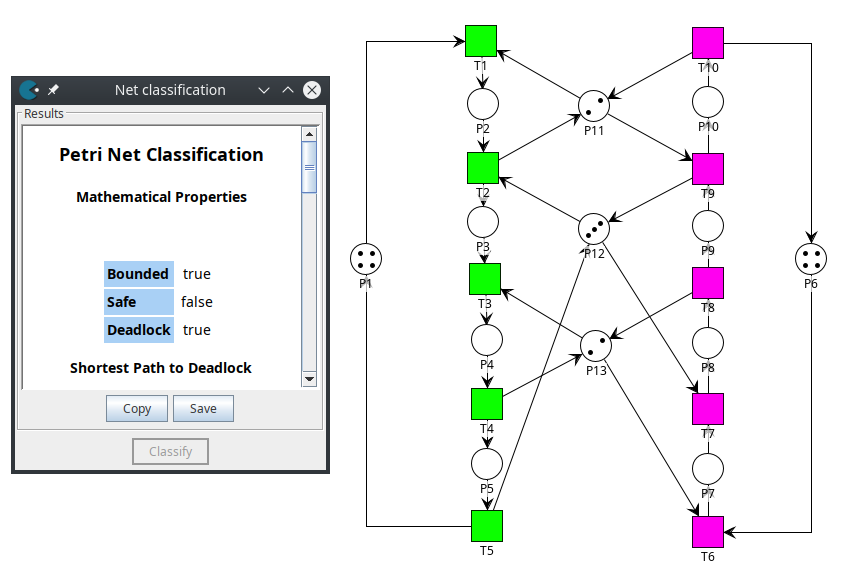
\includegraphics[width=\textwidth]{Figures/testing/yifan2_tinvariantes.png}
	\caption[RdP YiFan2 y sus T-invariantes.]{RdP YiFan2 \footnotemark \ y sus T-invariantes.}
	\label{fig:yifan2_invariantes}
 \end{figure} \footnotetext{Figura adaptada del paper publicado por \textit{YiFan Hou} et al. \cite{paperyifanhou}}

En la figura \ref{fig:yifan2_invariantes}, se presentan los T-invariantes en diferentes colores. \\


\paragraph{Control de la red}
\hfill \break
Para alcanzar la vivacidad de esta red bastó con agregar los supervisores y no fue necesario ejecutar la parte 3 del algoritmo dado que al agregar los mismos se alcanzó el control de la red, eliminando las situaciones de deadlock.
\begin{table}[H]
    \small
    \centering
    \begin{tabular}{|c|c|P{2cm}|P{2.3cm}|c|}
    \hline
    \textbf{Supervisor} & \textbf{Marcado} & \textbf{Transiciones input} & \textbf{Transiciones output} & \textbf{Bad Siphon Controlado}  \\  \hline
    $P_{14}$ & 6 & \{$T_{4},T_{9}$\} & \{$T_{1},T_{6}$\} & \{$P_4, P_5, P_8, P_{10}, P_{11}, P_{12}, P_{13}$\} \\ 
    \hline
    $P_{15}$ & 4 & \{$T_{4}, T_{8}$\} & \{$T_1,T_6$\} & \{$P_4, P_5, P_{8}, P_{9}, P_{12}, P_{13}$\} \\ 
    \hline
    $P_{16}$ & 4 & \{$T_{2}, T_{9}$\} & \{$T_1,T_6$\} & \{$P_3, P_4, P_{5}, P_{10}, P_{11}, P_{12}$\} \\
    \hline
    \end{tabular}
    \caption{Supervisores: RdP YiFan2}
    \label{tab:Yifan2}
\end{table}
\hfill

\begin{figure}[H]
	\centering
	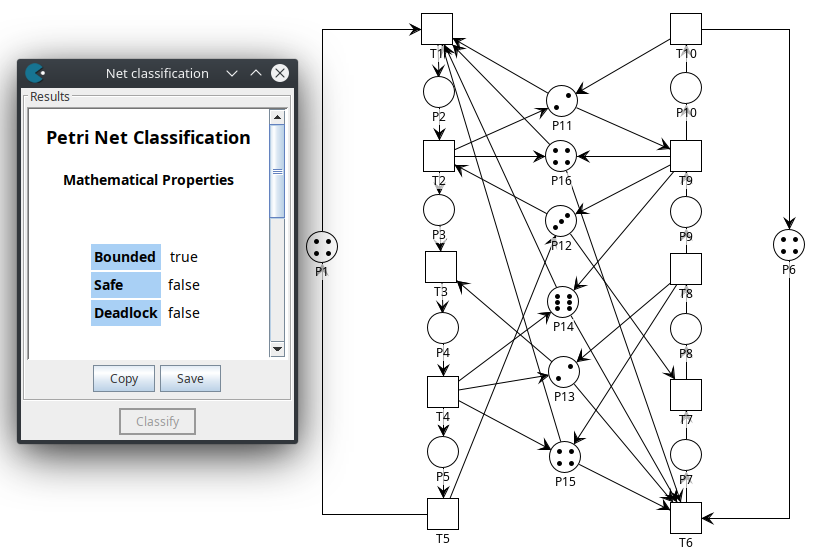
\includegraphics[width=\textwidth]{Figures/testing/yifan2_controlada.png}
	\caption[RdP YiFan2 controlada]{RdP YiFan2 controlada.}
	\label{fig:yifan2controlada}
 \end{figure}
 
 %-------------------------------------------------------------------------------------
\subsubsection{Características generales YiFan3}
\begin{itemize}
    \item Los recursos de la red están representados por las plazas \{$P_{5},P_{6}$\}.
\end{itemize}

\subsubsection{Análisis estructural YiFan3}
\hfill
\begin{figure}[H]
	\centering
	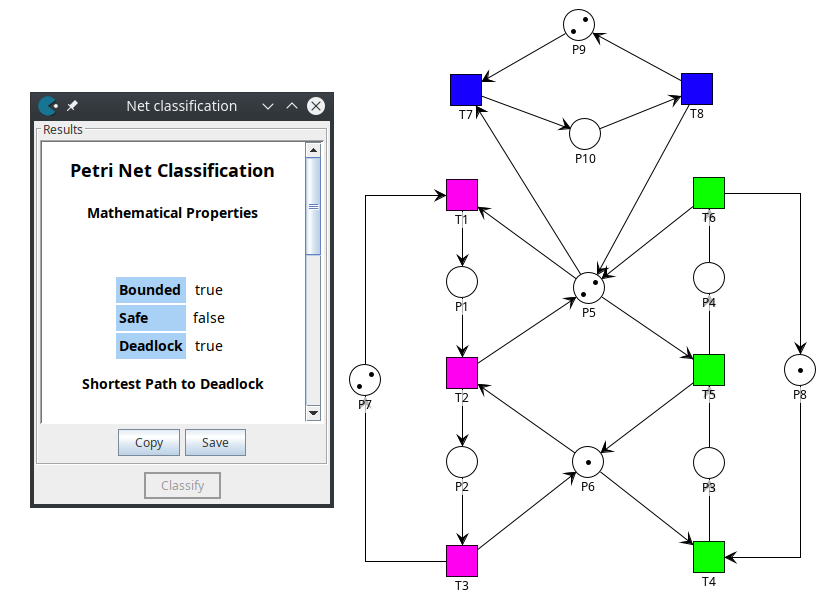
\includegraphics[width=\textwidth]{Figures/testing/yifan3_tinvariantes.png}
	\caption[RdP YiFan3 y sus T-invariantes.]{RdP YiFan3 \footnotemark \ y sus T-invariantes.}
	\label{fig:yifan3invariantes}
 \end{figure} \footnotetext{Figura adaptada del paper publicado por \textit{YiFan Hou} et al. \cite{paperyifanhou}}

En la figura \ref{fig:yifan3invariantes}, se presentan los T-invariantes en diferentes colores. \\

\paragraph{Control de la red}
\hfill \break
Al agregar los supervisores en la red ésta aún presentaba deadlock, lo que se hizo fue ejecutar la parte 3 del algoritmo para resolver tanto el problema de conflicto y de t\_idle, logrando de esta manera el control de la red.
\begin{table}[H]
    \small
    \centering
    \begin{tabular}{|c|c|P{2cm}|P{2.3cm}|c|}
    \hline
    \textbf{Supervisor} & \textbf{Marcado} & \textbf{Transiciones input} & \textbf{Transiciones output} & \textbf{Bad Siphon Controlado}  \\  \hline
    $P_{11}$ & 2 & \{$T_{2},T_{5}$\} & \{$T_{1},T_{4}$\} & \{$P_2, P_4, P_5,P_6, P_{10}$\} \\ 
    \hline
    \end{tabular}
    \caption{Supervisores: RdP YiFan3}
    \label{tab:Yifan3}
\end{table}
\hfill

\begin{figure}[H]
	\centering
	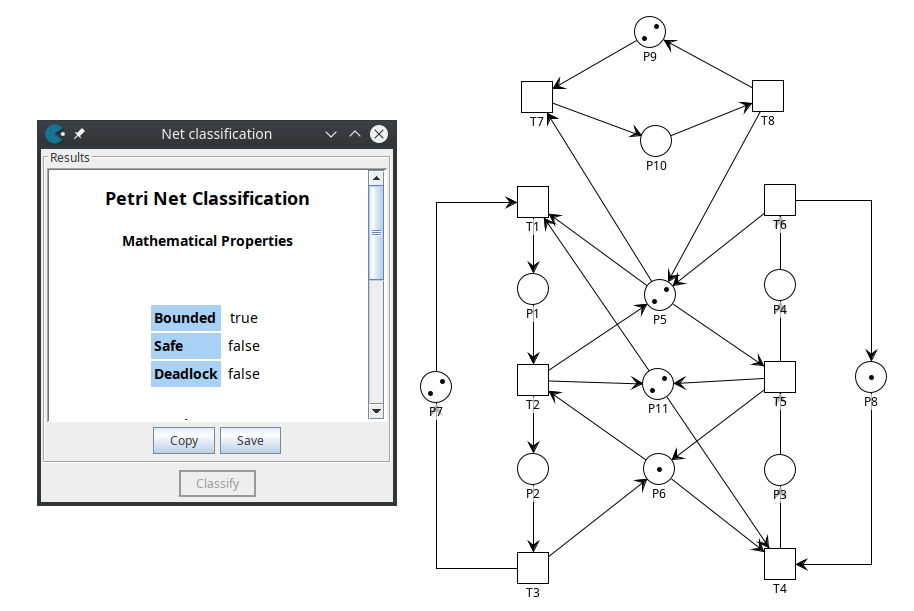
\includegraphics[width=\textwidth]{Figures/testing/yifan3_controlada.png}
	\caption[RdP YiFan3 controlada]{RdP YiFan3 controlada.}
	\label{fig:yifan3controlada}
 \end{figure}
 
 %-------------------------------------------------------------------------------------
\subsection{Caso JianChao}
Esta red modela la ejecución concurrente de un AMS, se presentan dos procesos productivos que comparten compuesto por 4 robot y 6 maquinas. Un control incorrecto de estos en la ejecución de los procesos de trabajo, puede conducir a situaciones de deadlock.\\

% \begin{figure}[H]
% 	\centering
% 	\includegraphics[width=\textwidth]{Figures/testing/jianchaomodelado.png}
% 	\caption[Modelado RdP JianChao.]{Modelado RdP JianChao \footnotemark \.}
% 	\label{fig:modeladoJianchao}
%  \end{figure} \footnotetext{Figura adaptada del paper publicado por \textit{H. Liu} et al. \cite{JianchaoModelado}}

\subsubsection{Características generales}
\begin{itemize}
    \item Los robot de la red están representados por las plazas \{$P_{20}, P_{22}, P_{24}, P_{26}$\}.
    \item Las maquinas de la red están representados por las plazas \{$P_{21}, P_{23}, P_{25}, P_{27}, P_{28}, P_{29}$\}.
\end{itemize}

\subsubsection{Análisis estructural}
\hfill
\begin{figure}[H]
	\centering
	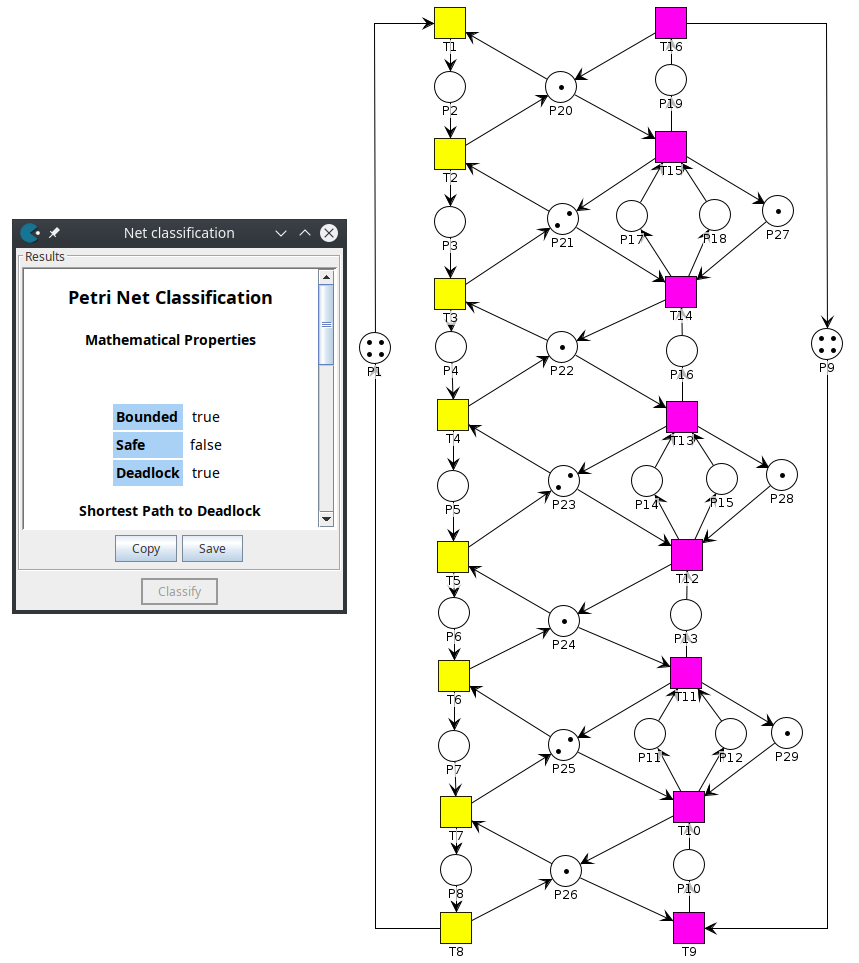
\includegraphics[width=\textwidth]{Figures/testing/jianchaodeadlock.png}
	\caption[RdP JianChao y sus T-invariantes.]{RdP JianChao \footnotemark \ y sus T-invariantes.}
	\label{fig:jianchaoinvariantes}
 \end{figure} \footnotetext{Figura adaptada del paper publicado por \textit{JianChao Lou} et al. \cite{paperjianchao}}

En la figura \ref{fig:jianchaoinvariantes} \footnote{En esta RdP fue modificado el peso de los arcos reduciéndolos a uno para adaptarlas al tipo de red que admite el algoritmo.}, se presentan los T-invariantes en diferentes colores.\\

\paragraph{Control de la red}
\hfill \break
Para alcanzar la vivacidad de esta red bastó con agregar los supervisores y no fue necesario ejecutar la parte 3 del algoritmo dado que al agregar los mismos se alcanzó el control de la red, eliminando las situaciones de deadlock.
\begin{table}[H]
    \small
    \centering
    \begin{tabular}{|c|c|P{2cm}|P{2.3cm}|c|}
    \hline
    \textbf{Supervisor} & \textbf{Marcado} & \textbf{Transiciones input} & \textbf{Transiciones output} & \textbf{Bad Siphon Controlado}  \\  \hline
    $P_{30}$ & 2 & \{$T_{7},T_{10}$\} & \{$T_{1},T_{9}$\} & \{$P_8, P_{11}, P_{25}, P_{26}$\} \\ 
    \hline
    $P_{31}$ & 2 & \{$T_{5}, T_{12}$\} & \{$T_1,T_9$\} & \{$P_6, P_{14}, P_{23}, P_{24}$\} \\ 
    \hline
    $P_{32}$ & 2 & \{$T_{3}, T_{14}$\} & \{$T_1,T_9$\} & \{$P_4, P_{17}, P_{21}, P_{22}$\} \\ 
    \hline
    \end{tabular}
    \caption{Supervisores: RdP JianChao}
    \label{tab:Jianchao}
\end{table}
\hfill

\begin{figure}[H]
	\centering
	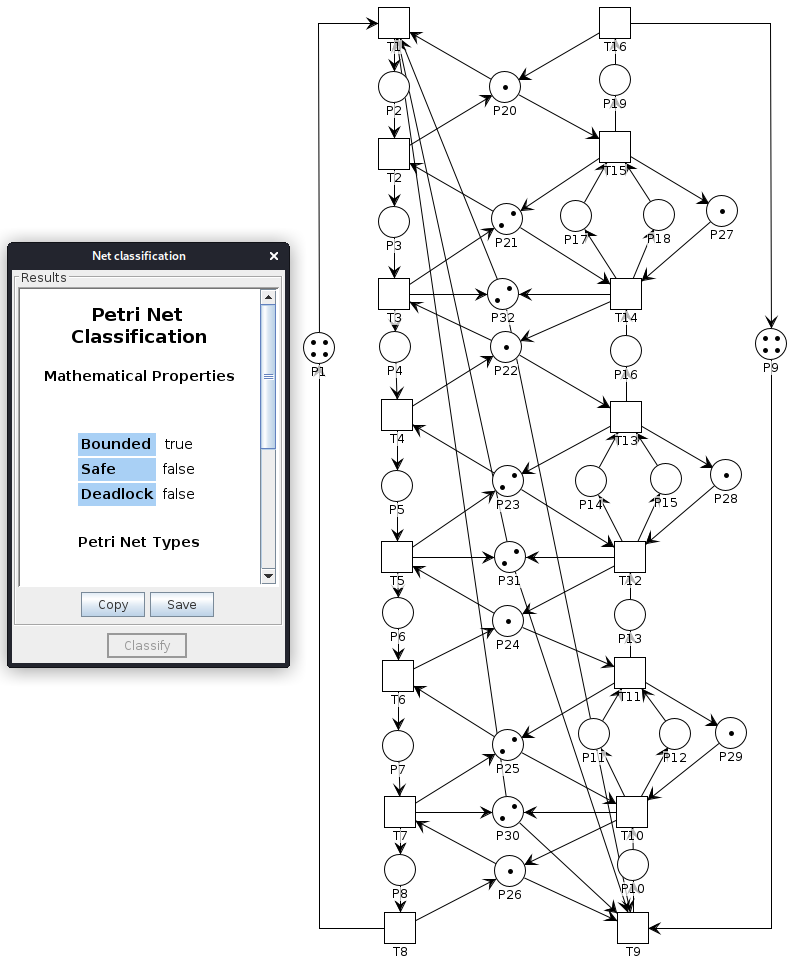
\includegraphics[width=\textwidth]{Figures/testing/jianchao_controlada.png}
	\caption[RdP JianChao controlada]{RdP JianChao controlada.}
	\label{fig:jianchaocontrolada}
 \end{figure}

%-------------------------------------------------------------------------------------

\subsection{Caso Zhiwuli}
Esta red modela la ejecución concurrente de un FMS. El mismo consta de 3 procesos productivos que comparten 2 recursos y un control incorrecto de estos en la ejecución de los procesos de trabajo, puede conducir a situaciones de deadlock.

\subsubsection{Características generales}
\begin{itemize}
    \item Los recursos de la red están representados por las plazas \{$P_{7},P_{8}$\}.
\end{itemize}

\subsubsection{Análisis estructural}
\hfill
\begin{figure}[H]
	\centering
	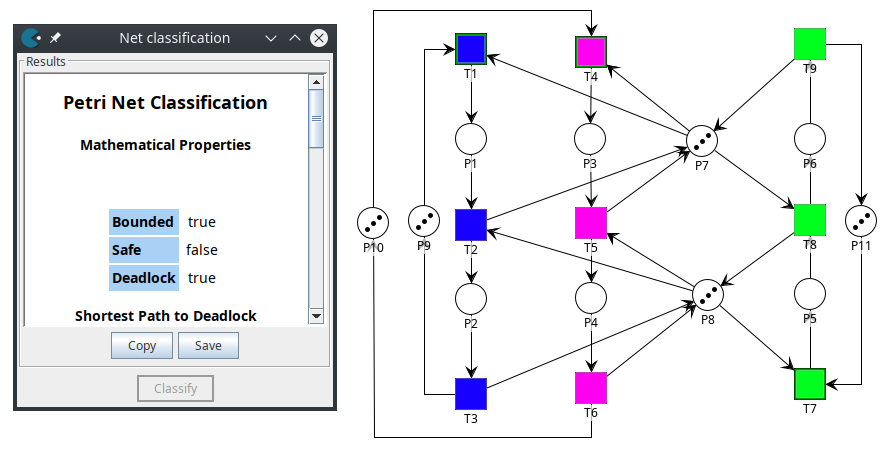
\includegraphics[width=\textwidth]{Figures/testing/zhiwuli_tinvariantes.png}
	\caption[RdP Zhiwuli y sus T-invariantes.]{RdP Zhiwuli \footnotemark \ y sus T-invariantes.}
	\label{fig:zhiwuli_tivariantes}
 \end{figure} \footnotetext{Figura adaptada del paper publicado por \textit{ZhiWu Li} et al. \cite{paperzhiwuli}}

En la figura \ref{fig:zhiwuli_tivariantes} \footnote{En esta RdP fue modificado el peso de los arcos reduciéndolos a uno (1) para adaptarla al tipo de red que admite el algoritmo.}, se presentan los T-invariantes en diferentes colores. \\

\paragraph{Control de la red}
\hfill \break
Para alcanzar la vivacidad de esta red bastó con agregar los supervisores y no fue necesario ejecutar la parte 3 del algoritmo dado que al agregar los mismos se alcanzó el control de la red, eliminando las situaciones de deadlock.

\bigskip
\begin{table}[H]
    \small
    \centering
    \begin{tabular}{|c|c|P{2cm}|P{2.3cm}|c|}
    \hline
    \textbf{Supervisor} & \textbf{Marcado} & \textbf{Transiciones input} & \textbf{Transiciones output} & \textbf{Bad Siphon Controlado}  \\  \hline
    $P_{12}$ & 5 & \{$T_{2}, T_5, T_{8}$\} &  \{$T_{1},T_{4}, T_7$\} & \{$P_2, P_4, P_6, P_7, P_8$\} \\ 
    \hline
    \end{tabular}
    \caption{Supervisores: RdP Zhiwuli}
    \label{tab:Zhiwuli}
\end{table}
\hfill

\begin{figure}[H]
	\centering
	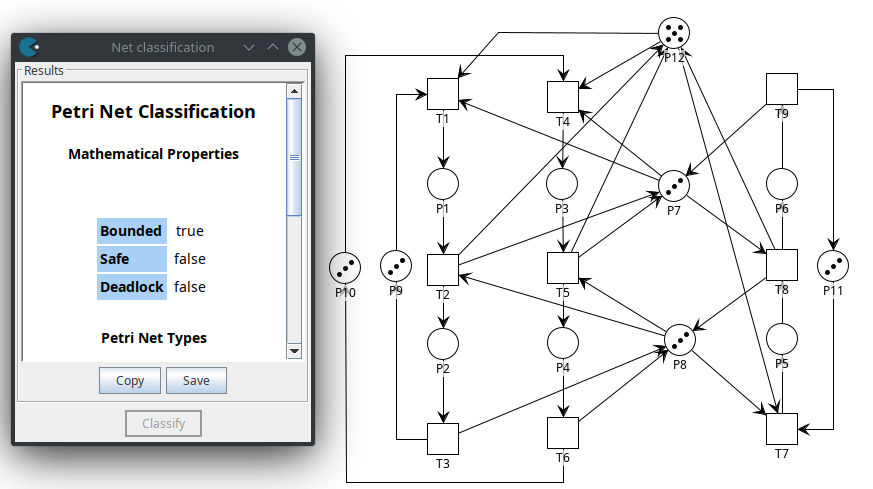
\includegraphics[width=\textwidth]{Figures/testing/zhiwuli_controlada.png}
	\caption[RdP Zhiwuli controlada]{RdP Zhiwuli controlada.}
	\label{fig:zhiwulicontrolada}
 \end{figure}
 
 %-------------------------------------------------------------------------------------
 
\subsection{Caso Fanti}
La red representa un AMS, la cual consta de un conjunto de estaciones de trabajo, cada una de las cuales es capaz de procesar piezas de diferente tipo de acuerdo con una secuencia de operaciones prescrita. Para el desarrollo de estas piezas la red presenta 4 recursos compartidos y una mala gestión de los mismos desencadenará el bloqueo de la red.

\subsubsection{Características generales}
\begin{itemize}
    \item Los recursos de la red están representados por las plazas \{$P_{10},P_{11},P_{12},P_{13}$\}.
\end{itemize}

\subsubsection{Análisis estructural}
\hfill
\begin{figure}[H]
	\centering
	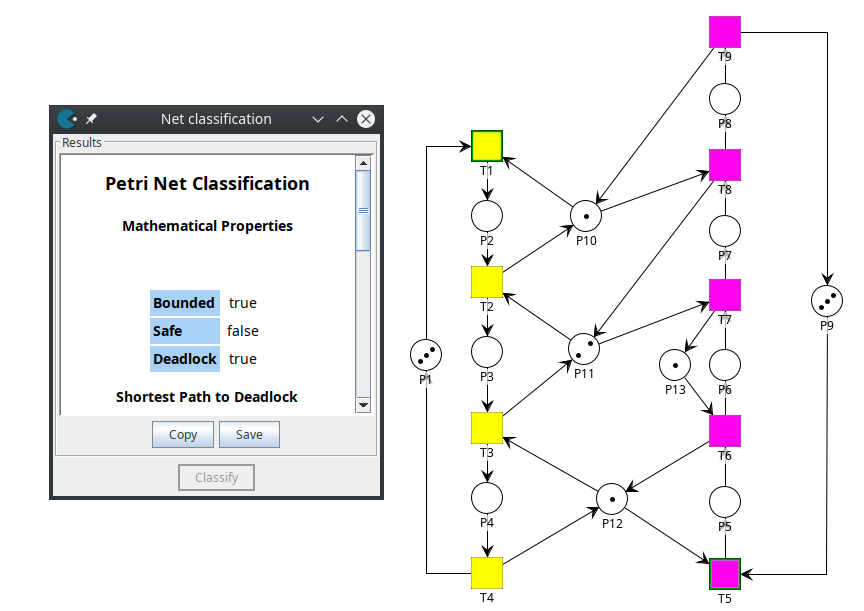
\includegraphics[width=\textwidth]{Figures/testing/fanti_tinvariantes.png}
	\caption[RdP Fanti y sus T-invariantes.]{RdP Fanti \footnotemark \ y sus T-invariantes.}
	\label{fig:fanti_tinvariantes}
 \end{figure} \footnotetext{Figura adaptada del paper publicado por \textit{Fanti} et al. \cite{paperfanti}}

En la figura \ref{fig:fanti_tinvariantes} , se presentan los T-invariantes en diferentes colores.\\

\paragraph{Control de la red}
\hfill \break
Para alcanzar la vivacidad de esta red bastó con agregar los supervisores y no fue necesario ejecutar la parte 3 del algoritmo dado que al agregar los mismos se alcanzó el control de la red, eliminando las situaciones de deadlock.
\begin{table}[H]
    \small
    \centering
    \begin{tabular}{|c|c|P{2cm}|P{2.3cm}|c|}
    \hline
    \textbf{Supervisor} & \textbf{Marcado} & \textbf{Transiciones input} & \textbf{Transiciones output} & \textbf{Bad Siphon Controlado}  \\  \hline
    $P_{14}$ & 4 & \{$T_{3},T_{8}$\} & \{$T_{1},T_{5}$\} & \{$P_4, P_8, P_{10}, P_{11}, P_{12}, P_{13} $\} \\ 
    \hline
    $P_{15}$ & 2 & \{$T_{2}, T_{8}$\} & \{$T_1,T_5$\} & \{$P_3, P_8, P_{10}, P_{11}$\} \\ 
    \hline
    $P_{16}$ & 3 & \{$T_{3}, T_{7}$\} & \{$T_1,T_5$\} & \{$P_4, P_7, P_{11}, P_{12}, P_{13}$\} \\ 
    \hline
    \end{tabular}
    \caption{Supervisores: RdP Fanti}
    \label{tab:fanti}
\end{table}
\hfill

\begin{figure}[H]
	\centering
	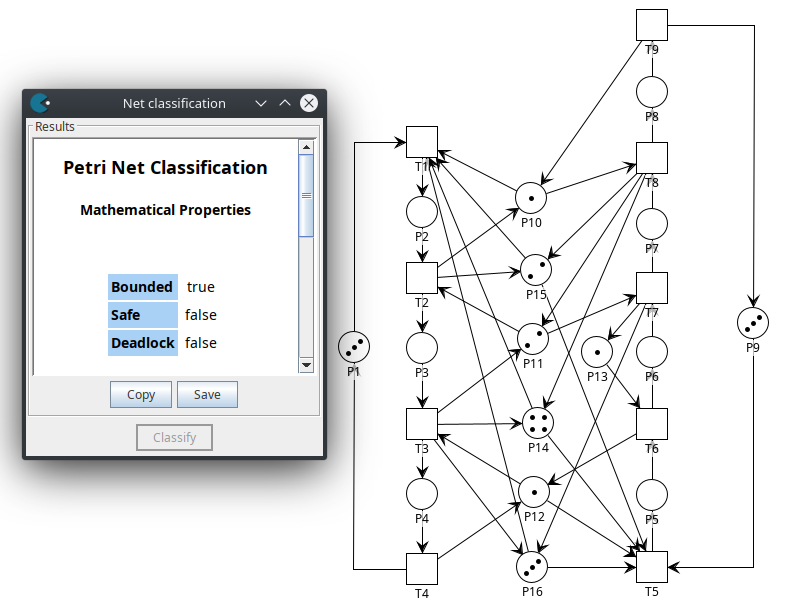
\includegraphics[width=\textwidth]{Figures/testing/fanti_controlada.png}
	\caption[RdP Fanti controlada]{RdP Fanti controlada.}
	\label{fig:fanticontrolada}
 \end{figure}
 
%-------------------------------------------------------------------------------------
\subsection{Caso Hesuan Hu}
La red representa un AMS donde se fabrican tres tipos de productos. El sistema esta compuesto por seis robots y cinco maquinas, cada uno de estos puede contener un solo producto.

 \subsubsection{Características generales}
\begin{itemize}
    \item Los robots de la red están representados por las plazas \{$P_{20},P_{22},P_{23},P_{30},P_{33},P_{35},$\}.
    \item Las máquinas de la red están representados por las plazas \{$P_{8},P_{9},P_{21},P_{31},P_{32}$\}.
    \item El primer producto comienza con la ejecución de la {$T_1$} y finaliza con la {$T_4$}.
    \item El segundo producto comienza con la ejecución de la {$T_9$} y finaliza con la {$T_{14}$}.
    \item El tercer producto comienza con la ejecución de la {$T_{19}$} y finaliza con la {$T_{24}$}.
\end{itemize}

\subsubsection{Análisis estructural}
\hfill
\begin{figure}[H]
	\centering
	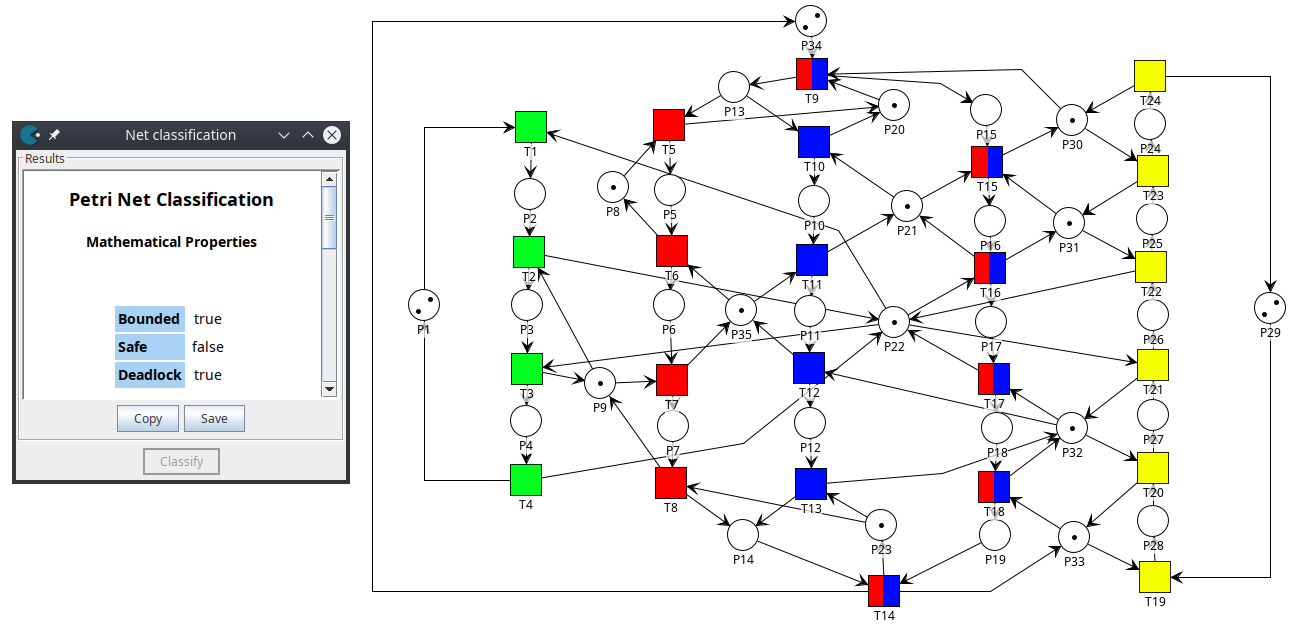
\includegraphics[width=\textwidth]{Figures/testing/fig3_deadlock.png}
	\caption[RdP Hesuan Hu y sus T-invariantes.]{RdP Hesuan Hu \footnotemark \ y sus T-invariantes.}
	\label{fig:hesuan_hu_tinvariantes}
 \end{figure} \footnotetext{Figura adaptada del paper publicado por \textit{Hesuan Hu} et al. \cite{paperhu}}

En la figura \ref{fig:hesuan_hu_tinvariantes} \footnote{En esta RdP fue modificado el peso de los arcos reduciéndolos a uno para adaptarlas al tipo de red que admite el algoritmo.}, se presentan los T-invariantes en diferentes colores.\\

\paragraph{Control de la red}
\hfill \break
Al agregar los supervisores en la red ésta aún presentaba deadlock, lo que se hizo fue ejecutar la parte 3 del algoritmo para resolver tanto el problema de conflicto y de t\_idle, logrando de esta manera el control de la red.
\begin{table}[H]
    \small
    \centering
    \begin{tabular}{|c|c|P{2.4cm}|P{2.2cm}|P{4.2cm}|}
    \hline
    \textbf{Supervisor} & \textbf{Marcado} & \textbf{Transiciones input} & \textbf{Transiciones output} & \textbf{Bad Siphon Controlado}  \\  \hline
    $P_{36}$ & 2 & \{$T_{3},T_{16},T_{22}$\} & \{$T_{1},T_{9},T_{19}$\} & \{$P_4, P_7, P_{9}, P_{17}, P_{22}, P_{25}, P_{31} $\} \\ 
    \hline
    $P_{37}$ & 1 & \{$T_{17}, T_{21}$\} & \{$T_9,T_{19}$\} & \{$P_2, P_4, P_{12}, P_{18}, P_{22}, P_{26}, P_{32}$\} \\ 
    \hline
    $P_{38}$ & 3 & \{$T_{3}, T_{8}, T_{13}, T_{21}$\} & \{$T_1,T_9, T_{19}$\} & \{$P_4, P_7, P_{9}, P_{12}, P_{14}, P_{22}, P_{26}, \break P_{32}, P_{33}$\} \\ 
    \hline
    $P_{39}$ & 1 & \{$T_{3}$\} & \{$T_1$\} & \{$P_4, P_7, P_{9}, P_{17}, P_{22}, P_{26}$\} \\ 
    \hline
    $P_{40}$ & 1 & \{$T_{16}, T_{22}$\} & \{$T_9,T_{19}$\} & \{$P_2, P_4, P_{17}, P_{22}, P_{25}, P_{31}$\} \\ 
    \hline
    \end{tabular}
    \caption{Supervisores: RdP Hesuan Hu}
    \label{tab:hu}
\end{table}
\hfill

\begin{figure}[H]
	\centering
	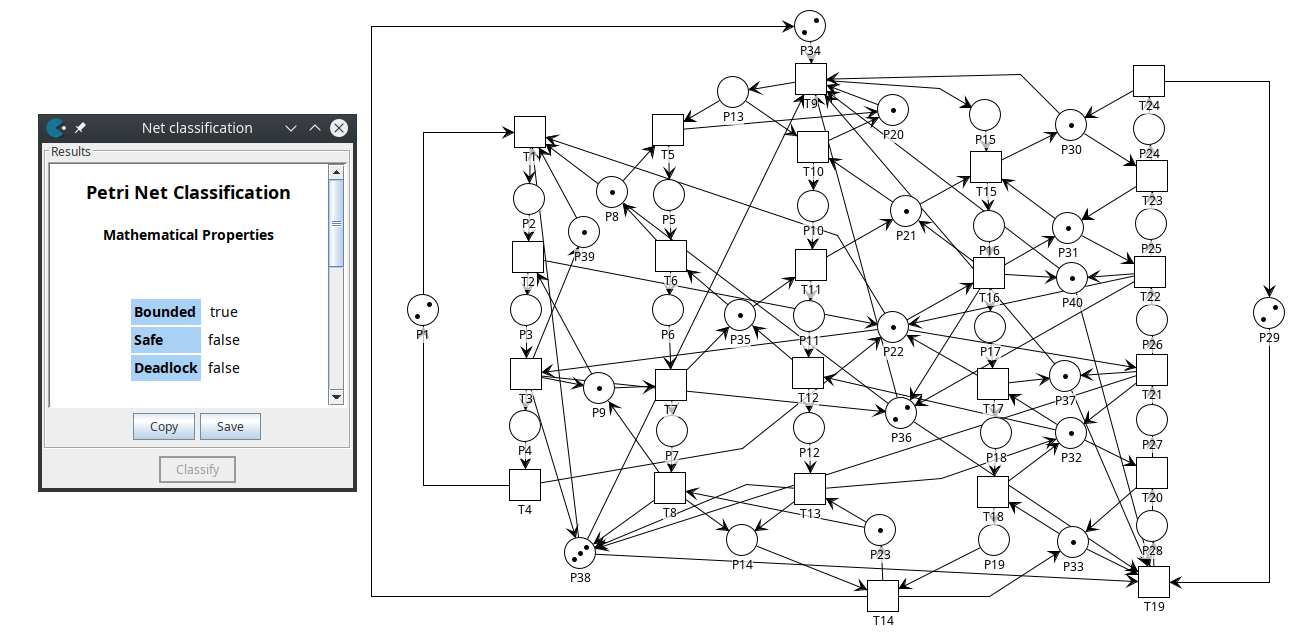
\includegraphics[width=\textwidth]{Figures/testing/fig3_sindeadlock.png}
	\caption[RdP Hesuan Hu controlada]{RdP Hesuan Hu controlada.}
	\label{fig:hucontrolada}
 \end{figure}